\subchapter{Kernel optimizations}{Measure kernel boot components and
optimize the kernel boot time}

\section{Measuring}

We are going to use the kernel \code{initcall_debug} functionality.

Our default kernel already has the configuration settings that we need:
\begin{itemize}
\item \kconfigval{CONFIG_PRINTK_TIME}{y}, to add a timestamp to each kernel
message.
\item \kconfigval{CONFIG_LOG_BUF_SHIFT}{16}, to have a big enough kernel ring buffer.
\end{itemize}

That's not sufficient. We also need the output of the \code{dmesg}
command.

We are going to make a few changes to the root filesystem. To save time
later going back to the initial Buildroot configuration, make a copy
of the \code{buildroot/} directory to \code{buildroot-dmesg/}:

\begin{verbatim}
cp -al buildroot/ buildroot-dmesg/
\end{verbatim}

In this new directory, add support for \code{dmesg} command in BusyBox,
and add the below line after the \code{ffmpeg} line in the
\code{playvideo} scripts:

\begin{verbatim}
dmesg > /dev/console
\end{verbatim}

Run Buildroot again, and update your
\code{~/boot-time-labs/rootfs/rootfs} directory again. Compile your
kernel again to to update the \code{zImage} with this root filesystem.

Now, let's enable \code{initcall_debug} in kernel parameters. Go to
the U-Boot command line, and add the below settings to the kernel command line
\footnote{Don't save these settings with \code{saveenv}. We
will just need them once.}, and boot your system:
\begin{verbatim}
setenv bootargs ${bootargs} initcall_debug printk.time=1
boot
\end{verbatim}

Boot the board with the new kernel image. If everything went well,
you can now copy and paste the special \code{dmesg} output to
a \code{~/boot-time-labs/kernel/initcall_debug.log} file on your workstation.

In \code{~/boot-time-labs/kernel} (at least where the kernel sources
are), run the following command to generate a boot graph:

\begin{verbatim}
linux/scripts/bootgraph.pl initcall_debug.log > boot.svg
\end{verbatim}

You can view the boot graph with the \code{inkscape} vector graphics
editor:

\begin{verbatim}
sudo apt install inkscape
inkscape boot.svg
\end{verbatim}

\begin{center}
\includegraphics[width=\textwidth]{labs/boot-time-kernel/boot.pdf}
\end{center}

Now review the longest initcalls in detail. Each label is the name of
a function in the kernel sources. Try to find out in which source file
each function is defined\footnote{You can do it with utilities such as
\code{cscope}, which your instructor will be happy to demonstrate,
or through our on-line service to explore the Linux kernel sources:
\url{https://elixir.bootlin.com}}, and what each driver corresponds
to.

Then, you can look the source code and:
\begin{itemize}
\item See whether you need the corresponding driver or feature at all.
If that's the case, just disable it.
\item Otherwise, try look for obvious causes which
would explain the very long execution time: delay loops (look for
\code{delay}, parameters which can reduce probe time but are not used,
etc).
\item There could also be features than could be postponed.
However, in our special case, we should
only need to keep kernel features that we need to run our video player.
However, in a real life system, the boot graph could indeed reveal
drivers which could be compiled as modules and loaded later.
\end{itemize}

Recompile and reboot the kernel, updating the boot graph until there is
nothing left that you can do.

When you are done exploiting data from the boot graphs, resume
to using the root filesystem generated by the normal \code{buildroot}
workspace. Also remove \code{initcall_debug} and \code{printk.time=1}
from the kernel command line.

{\bf Note}: unfortunately, in recent kernels, at least for the BeagleBone Black
board, the boot graph no longer shows individual driver or device
related elapsed time. We haven't managed yet to find why
and how to get more useful bootgraphs again. So, our best solution is
to remove unnecessary functionality from the kernel, and keep an eye
on the timing of messages in the console, to detect what's taking most
time in the kernel initialization. That's almost equivalent, but more
manual.

\section{Optimizing necessary functionality - Delay loop calibration}

Take three measures of the boot time and store them in the first row of
the \code{boot-time-labs/results/lpj-time.ods} spreadsheet:

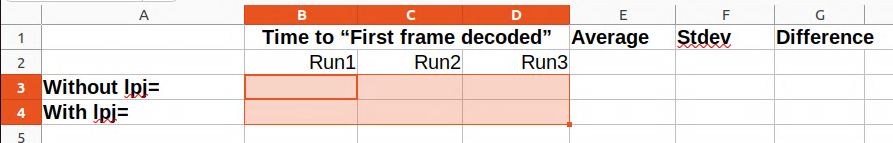
\includegraphics[width=0.7\textwidth]{labs/boot-time-kernel/lpj-time.png}

Implement the {\em Preset loops per jiffy} optimization by
finding the \code{lpj} value and adding it to the kernel command line.

Take three measures again and store them in the spreadsheet, to compute
the saved time.

\section{Removing unnecessary functionality}

It's time to start simplifying the kernel by remove drivers and features
that you won't need.

Do this {\bf very progressively}. If you go too fast, you'll end up with a
kernel that doesn't boot any more, but you won't be able to tell which
parameter should have been kept.

Also, don't disable \kconfig{CONFIG_PRINTK} too early
as you would lose all the kernel messages in the console.

Also, for the moment, don't touch the options related to size and
compression, including compiling the kernel with {\em Thumb2}, as the
impact of each option could depend on the size of the kernel.

Make sure you go through all the possibilities covered in the slides, in
particular to enable \kconfig{CONFIG_EMBEDDED} to allow to unselect further
features that should be present on a general purpose
system\footnote{Here we have a very specific system and we don't have
to support programs that could be added in the future and could need
more kernel features}.

You can even try to remove support for the \code{proc} and \code{sysfs}
filesystems, as we're not mounting them anyway. Surprisingly, at least
in our application and kernel, you'll see that the application doesn't
work if the \code{proc} filesystem is not compiled in. Let's keep that
one!

At the end, you can disable \kconfig{CONFIG_PRINTK}, and observe your
total savings in terms of kernel size and boot time.

Last but not least, try to find other ways of reducing the kernel size.
Go through the \code{.config} file and the kernel build log and look for
ideas to further reduce size and boot time.

\section{Optimizing required functionality}

The time has come to make final optimizations on our kernel, mainly
related to code size.

\subsection{Kernel instruction set}

First, measure and write down your kernel size and the total boot time
in the \code{~/boot-time-labs/results/kernel-size-arm-thumb2.ods} spreadsheet:

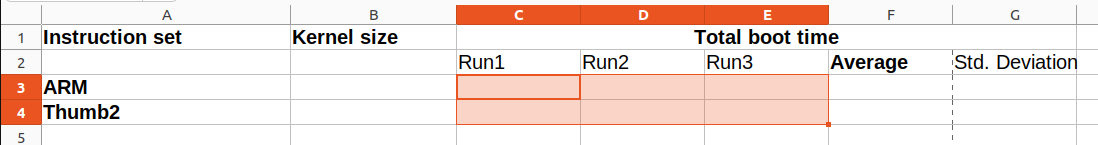
\includegraphics[width=\textwidth]{labs/boot-time-kernel/kernel-size-arm-thumb2.png}

Now, compile your kernel with \kconfig{CONFIG_THUMB2_KERNEL}. Before you do
this, you could make a backup copy of your kernel source directory with
\code{cp -al}, as a full rebuild of the kernel will be needed, and we
may want to roll back later. Fortunately, thanks to our feature
reduction work, the full rebuild should be faster than in the earlier labs.

Write down the kernel size and total boot time in the above table,
and keep whatever option works best for you.

\subsection{Kernel compression}

Install the below packages:

\begin{verbatim}
sudo apt install lzop lz4
\end{verbatim}

We are now going to try all the kernel compression schemes listed in
the \code{~/boot-time-labs/results/kernel-size-compression.ods} spreadsheet:

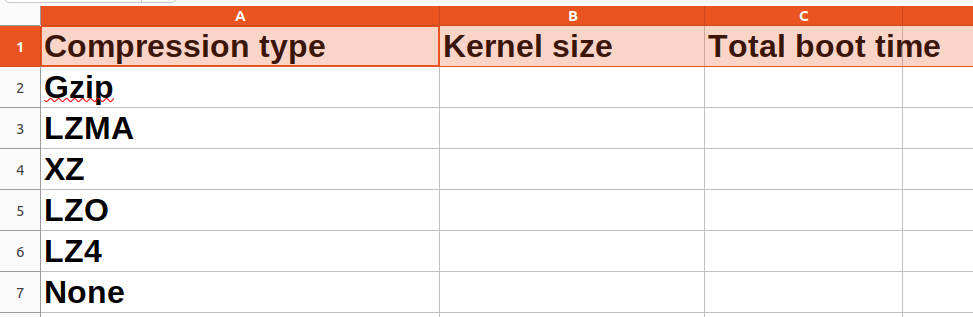
\includegraphics[width=\textwidth]{labs/boot-time-kernel/kernel-size-compression.png}

For the \code{None} row, there is no kernel configuration option, but
all you have to do is take the \code{arch/arm/boot/Image} file, and make a
\code{uImage} file out of it (as U-Boot's \code{bootz} command only
works with \code{zImage} files):

\begin{verbatim}
sudo apt install u-boot-tools
mkimage -A arm -O linux -C none  -T kernel -a 80008000 -e 80008000 \
        -n 'Linux' -d arch/arm/boot/Image arch/arm/boot/uImage
\end{verbatim}

Then, in U-Boot, you will have to boot it with \code{bootm} instead of
\code{bootz}.

This option can make sense when the CPU is very slow and the storage is
quite fast (like when you're booting Linux on a CPU emulated on an FPGA).

At the end, keep the option that gives you the best boot time, and
update the \code{~/boot-time-labs/results/kernel-optimizations.ods}
spreadsheet:

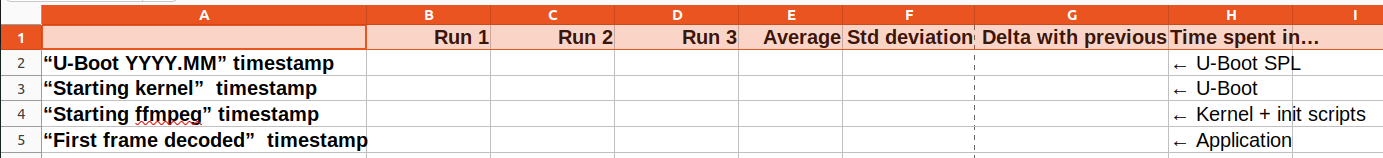
\includegraphics[width=\textwidth]{labs/boot-time-kernel/kernel-optimizations.png}

Note that we have merged the {\em Kernel} and {\em Init scripts} parts
(the latter being very short anyway), because the kernel is now silent.

At the end of this lab, you can remove the \code{buildroot-dmesg}
directory, which is no longer needed.
